% ============================================================
%  FLAER — Product & Technical Whitepaper
%  Compile with: pdflatex flaer_whitepaper.tex (run twice)
% ============================================================
\documentclass[11pt, a4paper]{article}

% ── Packages ────────────────────────────────────────────────
\usepackage[top=2.4cm, bottom=2.4cm, left=2.8cm, right=2.8cm]{geometry}
\usepackage{fontenc}
\usepackage{inputenc}
\usepackage{microtype}
\usepackage{parskip}
\usepackage{titlesec}
\usepackage{titling}
\usepackage{xcolor}
\usepackage{booktabs}
\usepackage{tabularx}
\usepackage{array}
\usepackage{colortbl}
\usepackage{enumitem}
\usepackage{graphicx}
\usepackage{hyperref}
\usepackage{fancyhdr}
\usepackage{tikz}
\usepackage{pgfplots}
\usepackage{listings}
\usepackage{tcolorbox}
\usepackage{multicol}
\usepackage{mdframed}
\usepackage{amsmath}
\usepackage{makecell}
\usepackage{pifont}

\pgfplotsset{compat=1.18}
\usetikzlibrary{positioning, arrows.meta, shapes, fit, backgrounds}
\tcbuselibrary{skins, breakable}

% ── Colours ─────────────────────────────────────────────────
\definecolor{flaergreen}{RGB}{44, 173, 132}
\definecolor{flaerdark}{RGB}{9, 24, 15}
\definecolor{flaerblue}{RGB}{127, 174, 255}
\definecolor{flaeramber}{RGB}{183, 149, 99}
\definecolor{flaerred}{RGB}{211, 93, 92}
\definecolor{flaergray}{RGB}{90, 110, 100}
\definecolor{rowalt}{RGB}{245, 250, 248}
\definecolor{codebg}{RGB}{240, 246, 243}

% ── Hyperref ────────────────────────────────────────────────
\hypersetup{
  colorlinks = true,
  linkcolor  = flaergreen,
  urlcolor   = flaergreen,
  citecolor  = flaergreen,
  pdftitle   = {Flaer — Product \& Technical Whitepaper},
  pdfauthor  = {Flaer},
}

% ── Section styling ─────────────────────────────────────────
\titleformat{\section}
  {\Large\bfseries\color{flaerdark}}
  {\color{flaergreen}\thesection}{0.8em}{}
  [\color{flaergreen}\titlerule]

\titleformat{\subsection}
  {\normalsize\bfseries\color{flaerdark}}
  {\color{flaergreen}\thesubsection}{0.6em}{}

\titleformat{\subsubsection}
  {\small\bfseries\color{flaergray}}
  {}{0em}{}

\titlespacing{\section}{0pt}{18pt}{8pt}
\titlespacing{\subsection}{0pt}{12pt}{4pt}

% ── Header / Footer ─────────────────────────────────────────
\pagestyle{fancy}
\fancyhf{}
\renewcommand{\headrulewidth}{0.4pt}
\renewcommand{\headrule}{\hbox to\headwidth{\color{flaergreen}\leaders\hrule height \headrulewidth\hfill}}
\fancyhead[L]{\small\color{flaergray}\textbf{flaer} \ · \ Sustainability Intelligence Platform}
\fancyhead[R]{\small\color{flaergray}Confidential}
\fancyfoot[C]{\small\color{flaergray}\thepage}

% ── Code listing style ───────────────────────────────────────
\lstset{
  backgroundcolor = \color{codebg},
  basicstyle      = \ttfamily\small,
  keywordstyle    = \color{flaergreen}\bfseries,
  commentstyle    = \color{flaergray}\itshape,
  stringstyle     = \color{flaeramber},
  breaklines      = true,
  frame           = single,
  rulecolor       = \color{flaergreen!40},
  framesep        = 4pt,
  xleftmargin     = 6pt,
  xrightmargin    = 6pt,
  aboveskip       = 8pt,
  belowskip       = 8pt,
}

% ── Info / Highlight boxes ───────────────────────────────────
\tcbset{
  flaerbox/.style = {
    enhanced, breakable,
    colback   = flaergreen!6,
    colframe  = flaergreen,
    fonttitle = \bfseries\small,
    coltitle  = white,
    attach boxed title to top left = {yshift=-2mm, xshift=4mm},
    boxed title style = {colback=flaergreen, rounded corners},
    arc = 3pt,
    boxrule = 0.6pt,
  },
  redbox/.style = {
    enhanced, colback=flaerred!6, colframe=flaerred,
    fonttitle=\bfseries\small, coltitle=white,
    attach boxed title to top left={yshift=-2mm,xshift=4mm},
    boxed title style={colback=flaerred,rounded corners},
    arc=3pt, boxrule=0.6pt,
  },
  bluebox/.style = {
    enhanced, colback=flaerblue!8, colframe=flaerblue,
    arc=3pt, boxrule=0.6pt,
  },
}

% ── Table helpers ────────────────────────────────────────────
\newcolumntype{L}[1]{>{\raggedright\arraybackslash}p{#1}}
\newcolumntype{C}[1]{>{\centering\arraybackslash}p{#1}}
\newcommand{\tableheader}[1]{\cellcolor{flaergreen!90}\textcolor{white}{\textbf{\small #1}}}
\newcommand{\greencheck}{\textcolor{flaergreen}{\textbf{\ding{51}}}}
\newcommand{\redcross}{\textcolor{flaerred}{\textbf{\ding{55}}}}
\newcommand{\partmark}{\textcolor{flaeramber}{\textbf{$\sim$}}}

% ────────────────────────────────────────────────────────────
\begin{document}

% ── Title page ──────────────────────────────────────────────
\begin{titlepage}
\pagecolor{flaerdark}
\color{white}
\vspace*{3cm}


\begin{tikzpicture}[remember picture, overlay]
  \fill[flaergreen] (0,0) rectangle (3pt, -28cm);
\end{tikzpicture}

\hspace{0.4cm}
\begin{minipage}{0.88\textwidth}
  {\fontsize{48}{52}\selectfont\bfseries\color{flaergreen} flaer}\\[0.3cm]
  {\Large\color{white!80} Sustainability Intelligence Platform}\\[2cm]

  {\LARGE\bfseries Product \& Technical Whitepaper}\\[0.5cm]
  {\large\color{white!60}
    Competitive positioning · Architecture · Data ingestion \\
    AI intelligence · Multi-tenancy · Go-to-market strategy
  }\\[3cm]

  \begin{tabular}{ll}
    \textcolor{flaergreen}{\textbf{Version}} & 1.0 \\[3pt]
    \textcolor{flaergreen}{\textbf{Date}}    & May 2026 \\[3pt]
    \textcolor{flaergreen}{\textbf{Status}}  & Confidential \\[3pt]
    \textcolor{flaergreen}{\textbf{Stack}}   & FastAPI · SvelteKit · SQLite/PostgreSQL · Groq LLM \\
  \end{tabular}

  \vspace{2cm}
  \color{white!40}\small
  This document contains proprietary and confidential information. Distribution or reproduction without written permission is prohibited.
\end{minipage}
\end{titlepage}

\nopagecolor
\color{black}

% ── Table of contents ───────────────────────────────────────
\newpage
\tableofcontents
\newpage

% ════════════════════════════════════════════════════════════
\section{Executive Summary}
% ════════════════════════════════════════════════════════════

\begin{tcolorbox}[flaerbox, title=One-line pitch]
\textit{``Flaer is the only platform built specifically for data center sustainability — covering today's compliance reporting, tomorrow's new builds, and the AI intelligence to connect both.''}
\end{tcolorbox}

\vspace{0.4cm}

Data center operators face three converging pressures that none of their current tools adequately address:

\begin{itemize}[leftmargin=1.4em]
  \item \textbf{€110/tCO$_2$e} carbon costs projected under EU ETS by 2030
  \item \textbf{Mandatory CSRD disclosure} for large EU-operating companies from FY2024
  \item \textbf{Board-level net-zero commitments} with no credible, auditable reporting pathway
\end{itemize}

Existing solutions fall into two categories: generic ESG platforms (Watershed, Persefoni, Salesforce Net Zero Cloud) that have no data center domain knowledge, or operational DCIM tools (Nlyte, Sunbird) that monitor uptime but produce no sustainability intelligence. \textbf{Flaer occupies the gap between them.}

The platform serves two distinct workflows in a single product: \textbf{operators} managing today's fleet of facilities, and \textbf{planners} selecting and evaluating locations for the next build. No competitor addresses both.

% ════════════════════════════════════════════════════════════
\section{The Market Problem}
% ════════════════════════════════════════════════════════════

\subsection{Regulatory Pressure}

The EU Corporate Sustainability Reporting Directive (CSRD) requires large companies to disclose:

\begin{itemize}[leftmargin=1.4em]
  \item Scope 1, 2 \& 3 greenhouse gas emissions (GHG Protocol aligned)
  \item Energy consumption breakdown and renewable energy mix
  \item Water withdrawal and consumption (WUE)
  \item EU Taxonomy alignment percentage of revenue, CapEx, and OpEx
  \item A credible 1.5°C-aligned transition plan
\end{itemize}

For data center operators, \textbf{Scope 2 (purchased electricity) typically represents 90--95\% of total emissions}. Getting this number right, with proper market-based vs location-based accounting, is mandatory — and most operators cannot do it today without expensive consultants.

\subsection{The Tool Gap}

\vspace{0.3cm}
\begin{tabular}{p{3cm} p{3.8cm} p{7.2cm}}
  \toprule
  \tableheader{Tool Category} & \tableheader{Examples} & \tableheader{What They Miss} \\
  \midrule
  Generic ESG platforms & Watershed, Persefoni, Salesforce Net Zero Cloud & No DC-specific metrics. PUE, WUE, CUE, grid carbon intensity, cooling type must be custom-configured. No site selection. \\
  \rowcolor{rowalt} DCIM / operational & Nlyte, Sunbird, Vertiv Trellis & No carbon forecasting, no CSRD output, no planning capability. Operational monitoring only. \\
  Manual spreadsheets & Excel, Google Sheets & No AI, no real-time data, no climate scenarios, no audit trail. \\
  \bottomrule
\end{tabular}

\vspace{0.5cm}

\begin{tcolorbox}[redbox, title=The Gap]
No existing product combines \textbf{real-time operational sustainability intelligence} with \textbf{new facility planning intelligence} for data centers. This is Flaer's market position.
\end{tcolorbox}

% ════════════════════════════════════════════════════════════
\section{Product Overview}
% ════════════════════════════════════════════════════════════

Flaer is a web-based SaaS platform built on FastAPI (Python backend) and SvelteKit (frontend), deployed as a single-tenant or multi-tenant cloud application. It provides eight core screens:

\vspace{0.3cm}
\begin{tabular}{p{3cm} p{3.2cm} p{7.8cm}}
  \toprule
  \tableheader{Screen} & \tableheader{Primary User} & \tableheader{Key Capability} \\
  \midrule
  Portfolio Overview & Sustainability Manager & Real-time PUE, WUE, CUE, carbon intensity per facility \\
  \rowcolor{rowalt} Forecast & Sustainability Manager & 2030/2035 emissions under SSP5-8.5 and optimised pathways \\
  Actions & Operations Lead & Ranked carbon \& cost reduction recommendations \\
  \rowcolor{rowalt} Facility Metrics & Operations Lead & Benchmarking, trending, and efficiency deep-dives \\
  Site Selection & Infrastructure Planner & 14-dimension MCDA scoring, risk matrix, financial model \\
  \rowcolor{rowalt} Comparison Report & Portfolio Manager & Facility-vs-facility across all sustainability dimensions \\
  flaer AI & All users & LLM assistant with live portfolio context \\
  \rowcolor{rowalt} Reports & Compliance Officer & CSRD-aligned PDF disclosure generation \\
  \bottomrule
\end{tabular}

\subsection{Operator Workflow}

For teams running existing data centers, Flaer provides:

\begin{itemize}[leftmargin=1.4em]
  \item \textbf{Anomaly detection} — automatic flagging when PUE $>$ 1.75 or WUE $>$ 1.8 L/kWh
  \item \textbf{Scope 2 accounting} — market-based and location-based calculations side by side
  \item \textbf{CSRD dashboard} — EU Taxonomy alignment status, disclosure readiness score
  \item \textbf{Weekly AI digest} — consumption summary with top 3 ranked actions
  \item \textbf{Carbon cost exposure} — EU ETS liability projection to 2030 and 2035
\end{itemize}

\subsection{Planner Workflow}

For teams evaluating new facility locations:

\begin{itemize}[leftmargin=1.4em]
  \item \textbf{Multi-Criteria Decision Analysis (MCDA)} across 14 weighted dimensions
  \item \textbf{Phase-gate workflow}: Screening $\rightarrow$ Pre-Feasibility $\rightarrow$ Risk Assessment $\rightarrow$ Financial Model
  \item \textbf{5$\times$5 risk matrix} with likelihood/impact scoring and mitigation plans
  \item \textbf{Financial model}: CapEx, OpEx, IRR, NPV, simple payback
  \item \textbf{Gantt timeline}: permitting, construction, commissioning
  \item \textbf{Due diligence report}: one-click PDF generation
\end{itemize}

% ════════════════════════════════════════════════════════════
\section{Competitive Differentiation}
% ════════════════════════════════════════════════════════════

\subsection{Positioning Map}

\begin{center}
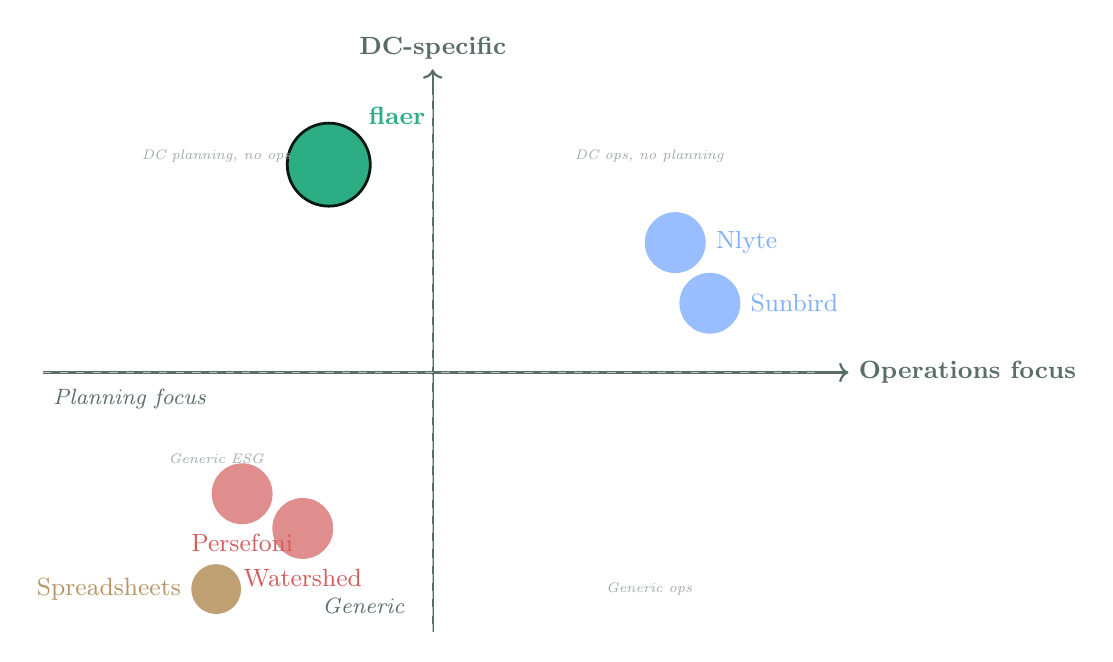
\begin{tikzpicture}[scale=1.1]
  % Axes
  \draw[->, thick, color=flaergray] (-4.5,0) -- (4.8,0)
    node[right, font=\small\bfseries, color=flaergray] {Operations focus};
  \draw[->, thick, color=flaergray] (0,-3) -- (0,3.5)
    node[above, font=\small\bfseries, color=flaergray] {DC-specific};

  \draw[dashed, color=flaergray!40] (-4.5,0) -- (4.5,0);
  \draw[dashed, color=flaergray!40] (0,-3) -- (0,3.2);

  % Labels
  \node[font=\footnotesize\itshape, color=flaergray] at (-3.5,-0.3) {Planning focus};
  \node[font=\footnotesize\itshape, color=flaergray] at (-0.8,-2.7) {Generic};

  % Competitors
  \node[circle, fill=flaerred!70, minimum size=22pt,
        label={[font=\small, color=flaerred]below:Watershed}] at (-1.5,-1.8) {};
  \node[circle, fill=flaerred!70, minimum size=22pt,
        label={[font=\small, color=flaerred]below:Persefoni}] at (-2.2,-1.4) {};
  \node[circle, fill=flaerblue!80, minimum size=22pt,
        label={[font=\small, color=flaerblue]right:Nlyte}] at (2.8,1.5) {};
  \node[circle, fill=flaerblue!80, minimum size=22pt,
        label={[font=\small, color=flaerblue]right:Sunbird}] at (3.2,0.8) {};
  \node[circle, fill=flaeramber!90, minimum size=18pt,
        label={[font=\small, color=flaeramber]left:Spreadsheets}] at (-2.5,-2.5) {};

  % Flaer
  \node[circle, fill=flaergreen, minimum size=30pt, draw=flaerdark, line width=1pt,
        label={[font=\small\bfseries, color=flaergreen]above right:flaer}] at (-1.2, 2.4) {};

  % Quadrant labels
  \node[font=\tiny\itshape, color=flaergray!60] at (2.5, 2.5) {DC ops, no planning};
  \node[font=\tiny\itshape, color=flaergray!60] at (-2.5, 2.5) {DC planning, no ops};
  \node[font=\tiny\itshape, color=flaergray!60] at (2.5, -2.5) {Generic ops};
  \node[font=\tiny\itshape, color=flaergray!60] at (-2.5, -1) {Generic ESG};
\end{tikzpicture}
\end{center}

\subsection{Feature Comparison Matrix}

\begin{tabular}{>{\raggedright\arraybackslash}p{5.2cm}
                 >{\centering\arraybackslash}p{1.5cm}
                 >{\centering\arraybackslash}p{2.1cm}
                 >{\centering\arraybackslash}p{1.7cm}
                 >{\centering\arraybackslash}p{2.4cm}}
  \toprule
  \tableheader{Capability} &
  \tableheader{flaer} &
  \tableheader{Watershed} &
  \tableheader{Nlyte} &
  \tableheader{Spreadsheet} \\
  \midrule
  \rowcolor{rowalt}
  DC-native PUE / WUE / CUE          & \greencheck & \redcross   & \greencheck & \redcross   \\
  CSRD \& EU Taxonomy output          & \greencheck & \redcross   & \redcross   & \redcross   \\
  \rowcolor{rowalt}
  Scope 2 market-based accounting     & \greencheck & \greencheck & \redcross   & \partmark   \\
  Site selection MCDA                 & \greencheck & \redcross   & \redcross   & \redcross   \\
  \rowcolor{rowalt}
  Climate scenario forecasting        & \greencheck & \partmark   & \redcross   & \redcross   \\
  Risk register \& due diligence      & \greencheck & \redcross   & \redcross   & \redcross   \\
  \rowcolor{rowalt}
  AI assistant (portfolio-aware)      & \greencheck & \redcross   & \redcross   & \redcross   \\
  Financial model (IRR / NPV)         & \greencheck & \redcross   & \redcross   & \partmark   \\
  \rowcolor{rowalt}
  Facility comparison report          & \greencheck & \partmark   & \partmark   & \redcross   \\
  Real-time anomaly detection         & \greencheck & \redcross   & \greencheck & \redcross   \\
  \rowcolor{rowalt}
  Day-one setup (no consultants)      & \greencheck & \redcross   & \redcross   & \greencheck \\
  \bottomrule
\end{tabular}

\vspace{0.4cm}
\begin{tcolorbox}[bluebox, left=8pt, right=8pt, top=5pt, bottom=5pt]
\small\bfseries
\greencheck\ \ Full support \qquad
\partmark\ \ Partial / requires configuration \qquad
\redcross\ \ Not supported
\end{tcolorbox}

% ════════════════════════════════════════════════════════════
\section{Technical Architecture}
% ════════════════════════════════════════════════════════════

\subsection{Stack Overview}

\begin{center}
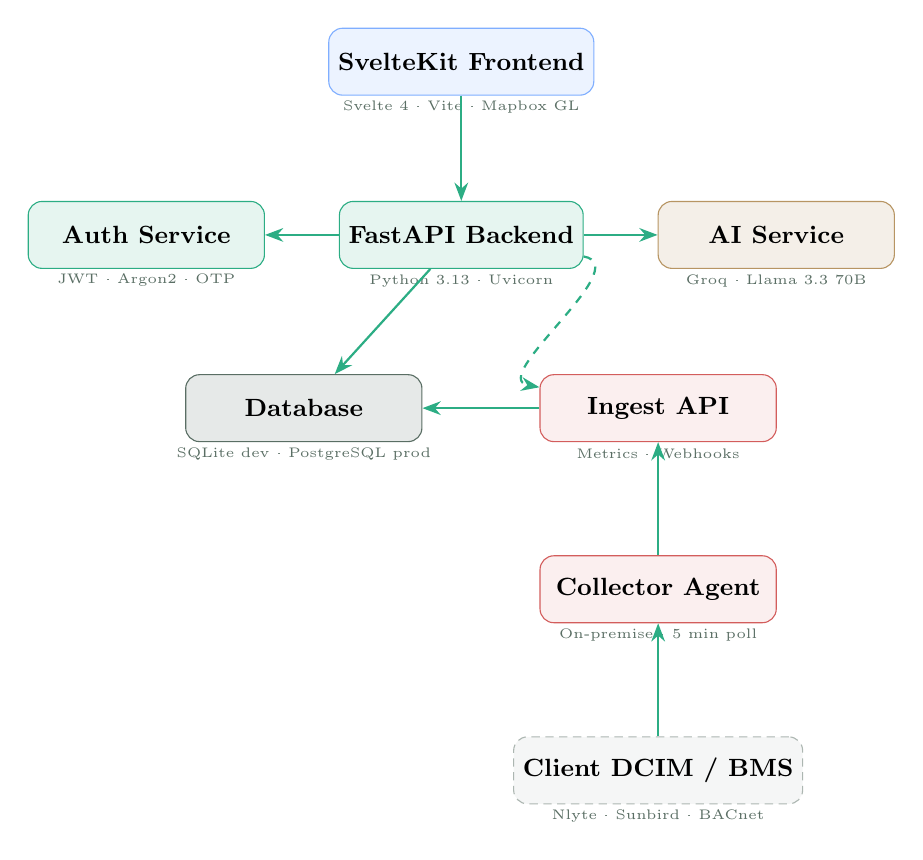
\begin{tikzpicture}[
  box/.style={rectangle, rounded corners=5pt,
              minimum width=3.0cm, minimum height=0.85cm,
              text centered, font=\small\bfseries, draw},
  lbl/.style={font=\tiny, color=flaergray},
  arr/.style={-Stealth, thick, color=flaergreen},
  darr/.style={-Stealth, thick, color=flaergreen, dashed}
]
  % Row 1 — Frontend (centred)
  \node[box, fill=flaerblue!15, draw=flaerblue]    (fe)  at (0, 6)    {SvelteKit Frontend};
  \node[lbl] at (0, 5.42) {Svelte 4 · Vite · Mapbox GL};

  % Row 2 — three service boxes, well-spaced
  \node[box, fill=flaergreen!12, draw=flaergreen]  (auth) at (-4, 3.8) {Auth Service};
  \node[lbl] at (-4, 3.22) {JWT · Argon2 · OTP};

  \node[box, fill=flaergreen!12, draw=flaergreen]  (api)  at (0, 3.8)  {FastAPI Backend};
  \node[lbl] at (0, 3.22) {Python 3.13 · Uvicorn};

  \node[box, fill=flaeramber!15, draw=flaeramber]  (ai)   at (4, 3.8)  {AI Service};
  \node[lbl] at (4, 3.22) {Groq · Llama 3.3 70B};

  % Row 3 — Database + Ingest
  \node[box, fill=flaergray!15, draw=flaergray]    (db)      at (-2, 1.6) {Database};
  \node[lbl] at (-2, 1.02) {SQLite dev · PostgreSQL prod};

  \node[box, fill=flaerred!10, draw=flaerred]      (ingest)  at (2.5, 1.6) {Ingest API};
  \node[lbl] at (2.5, 1.02) {Metrics · Webhooks};

  % Row 4 — Collector Agent
  \node[box, fill=flaerred!10, draw=flaerred]      (agent)   at (2.5, -0.7) {Collector Agent};
  \node[lbl] at (2.5, -1.28) {On-premise · 5 min poll};

  % Row 5 — Client DCIM (dashed)
  \node[box, fill=flaergray!6, draw=flaergray!50, densely dashed]
                                                    (dcim)    at (2.5, -3)  {Client DCIM / BMS};
  \node[lbl] at (2.5, -3.58) {Nlyte · Sunbird · BACnet};

  % Arrows
  \draw[arr]  (fe)     -- (api);
  \draw[arr]  (api)    -- (auth);
  \draw[arr]  (api)    -- (ai);
  \draw[arr]  (api)    -- (db);
  \draw[arr]  (ingest) -- (db);
  \draw[darr] (api)    to[out=-10, in=170] (ingest);
  \draw[arr]  (agent)  -- (ingest);
  \draw[arr]  (dcim)   -- (agent);
\end{tikzpicture}
\end{center}

\subsection{API Endpoints Reference}

\begin{tabular}{p{1.5cm} p{5.5cm} p{6.8cm}}
  \toprule
  \tableheader{Method} & \tableheader{Endpoint} & \tableheader{Description} \\
  \midrule
  POST & \texttt{/api/auth/register}        & Create account, returns JWT + refresh token \\
  \rowcolor{rowalt} POST & \texttt{/api/auth/login}            & Authenticate; returns JWT or OTP challenge \\
  POST & \texttt{/api/auth/verify-otp}       & Complete TOTP two-factor verification \\
  \rowcolor{rowalt} POST & \texttt{/api/auth/refresh}          & Rotate access token using refresh token \\
  GET  & \texttt{/api/auth/me}               & Return current user profile \\
  \rowcolor{rowalt} GET  & \texttt{/api/dashboard/overview}    & Portfolio KPIs (emissions, PUE, WUE, energy) \\
  GET  & \texttt{/api/dashboard/datacenters} & List all facilities for the authenticated org \\
  \rowcolor{rowalt} GET  & \texttt{/api/dashboard/forecast}    & 2030/2035 emissions forecast data \\
  GET  & \texttt{/api/dashboard/actions}     & Ranked carbon reduction action list \\
  \rowcolor{rowalt} POST & \texttt{/api/dashboard/calculator}  & Estimate emissions from input parameters \\
  GET  & \texttt{/api/carbon/live}           & Live grid carbon intensity (all regions) \\
  \rowcolor{rowalt} GET  & \texttt{/api/carbon/live/\{region\}}& Live grid carbon for a specific region \\
  GET  & \texttt{/api/ai/score-location/\{loc\}} & MCDA score for a candidate location \\
  \rowcolor{rowalt} POST & \texttt{/api/ai/recommend-locations}& Top-N location recommendations from requirements \\
  POST & \texttt{/api/ai/weekly-digest}      & Generate AI consumption digest for the org \\
  \rowcolor{rowalt} POST & \texttt{/api/ai/chat}               & LLM chat with live portfolio context (Groq) \\
  POST & \texttt{/api/ingest/metrics}        & Collector agent: push time-series facility data \\
  \rowcolor{rowalt} POST & \texttt{/api/data-centers}          & Register a new facility \\
  \bottomrule
\end{tabular}

\vspace{0.5cm}

\subsection{Deployment Model}

\begin{tabular}{p{2.8cm} p{3.5cm} p{7.8cm}}
  \toprule
  \tableheader{Environment} & \tableheader{Database} & \tableheader{Notes} \\
  \midrule
  Development  & SQLite (file-based)   & Zero-config local setup. \texttt{python main.py} starts the server. \\
  \rowcolor{rowalt} Staging      & PostgreSQL 15         & Full multi-tenant isolation. Mirrors production schema exactly. \\
  Production   & PostgreSQL 15 + TimescaleDB & TimescaleDB extension for efficient time-series queries on \texttt{facility\_metrics}. \\
  \bottomrule
\end{tabular}

\vspace{0.4cm}

All environments share the same codebase. The \texttt{DATABASE\_URL} environment variable switches between SQLite (\texttt{sqlite:///./flaer.db}) and PostgreSQL (\texttt{postgresql://...}) without any code change. Secrets (JWT key, Groq API key, Stripe key) are loaded from a \texttt{.env} file via \texttt{python-dotenv} and are never committed to the repository.

\subsection{Multi-Tenancy Model}

Every database record carries an \texttt{organization\_id} foreign key. All API endpoints filter by the authenticated user's organization — Client A can never access Client B's data, even if both share the same database instance.

\begin{lstlisting}[language=SQL, caption=Tenant isolation example]
-- All queries are scoped to the authenticated organization
SELECT * FROM data_centers
WHERE organization_id = :current_org_id
  AND is_active = 1;

-- Metrics table: time-series per facility per tenant
SELECT recorded_at, pue, wue, energy_mwh
FROM facility_metrics
WHERE org_id = :current_org_id
  AND dc_id  = :facility_id
ORDER BY recorded_at DESC
LIMIT 2016;  -- 1 week at 5-min intervals
\end{lstlisting}

\subsection{Authentication \& Security}

\begin{itemize}[leftmargin=1.4em]
  \item \textbf{JWT tokens} with 30-minute expiry and refresh token rotation
  \item \textbf{Argon2id} password hashing (OWASP recommended, PHC winner)
  \item \textbf{TOTP two-factor authentication} via PyOTP (RFC 6238)
  \item \textbf{Rate limiting} on all endpoints via SlowAPI
  \item \textbf{CSP headers} and HSTS enforced on all responses
  \item \textbf{Ingest API keys} scoped per facility, rotatable without affecting other tenants
\end{itemize}

% ════════════════════════════════════════════════════════════
\section{Real-Time Data Ingestion}
% ════════════════════════════════════════════════════════════

\subsection{The Problem}

A static PUE value stored once at onboarding tells you nothing about trends, anomalies, or weekly carbon accounting. Real sustainability intelligence requires \textbf{continuous time-series data per facility per tenant}.

\subsection{Time-Series Schema}

\begin{lstlisting}[language=SQL, caption=Facility metrics time-series table]
CREATE TABLE facility_metrics (
  id           TEXT PRIMARY KEY DEFAULT (hex(randomblob(8))),
  dc_id        TEXT    NOT NULL REFERENCES data_centers(id),
  org_id       TEXT    NOT NULL,                  -- tenant key
  recorded_at  DATETIME NOT NULL,
  pue          FLOAT,       -- Power Usage Effectiveness
  wue          FLOAT,       -- Water Usage Effectiveness (L/kWh)
  cue          FLOAT,       -- Carbon Usage Effectiveness
  energy_mwh   FLOAT,       -- Total facility energy
  it_load_kw   FLOAT,       -- IT equipment load
  cooling_kw   FLOAT,       -- Cooling system load
  temp_inlet   FLOAT,       -- Server inlet temperature (C)
  created_at   DATETIME DEFAULT CURRENT_TIMESTAMP
);

CREATE INDEX idx_fm_org_dc_time
  ON facility_metrics (org_id, dc_id, recorded_at DESC);
\end{lstlisting}

At 5-minute polling intervals, one facility generates \textasciitilde288 rows/day or \textasciitilde105,000 rows/year — manageable in SQLite for development, and trivially handled by PostgreSQL or TimescaleDB in production.

\subsection{Ingest API Endpoint}

\begin{lstlisting}[language=Python, caption=POST /api/ingest/metrics]
@app.post("/api/ingest/metrics")
async def ingest_metrics(payload: MetricsPayload,
                         api_key: str = Header(..., alias="X-API-Key"),
                         db: Session = Depends(get_db)):
    """
    Authenticated by per-facility API key (not user JWT).
    Called by the Collector Agent every 5 minutes.
    """
    facility = verify_ingest_key(api_key, db)   # raises 401 if invalid
    row = FacilityMetrics(
        dc_id       = facility.id,
        org_id      = facility.organization_id,
        recorded_at = payload.timestamp,
        pue         = payload.pue,
        wue         = payload.wue,
        energy_mwh  = payload.energy_mwh,
        it_load_kw  = payload.it_load_kw,
    )
    db.add(row)
    db.commit()
    return {"status": "ok", "recorded_at": payload.timestamp}
\end{lstlisting}

\textbf{Sample payload (JSON):}
\begin{lstlisting}[language={}]
POST /api/ingest/metrics
X-API-Key: flaer_ingest_a3f9c2...

{
  "facility_id": "virginia-dc-01",
  "timestamp":   "2026-05-13T14:30:00Z",
  "pue":         1.48,
  "wue":         0.74,
  "energy_mwh":  142.6,
  "it_load_kw":  96400,
  "temp_inlet":  21.3
}
\end{lstlisting}

\subsection{Ingestion Strategies by Client Type}

\begin{tabular}{p{3.2cm} p{3.5cm} p{5.8cm} p{1.6cm}}
  \toprule
  \tableheader{Client Type} & \tableheader{Method} & \tableheader{How It Works} & \tableheader{Effort} \\
  \midrule
  Modern DCIM (Nlyte, Sunbird) & Native integration (pull) & Flaer calls DCIM REST API on schedule; maps fields automatically & 1--2 weeks \\
  \rowcolor{rowalt} BMS with webhook support & Direct API push & Client configures BMS to POST to Flaer ingest endpoint on metric update & 1 day \\
  No modern integration & Collector Agent & Lightweight Python script on client server polls DCIM/BMS every 5 min and pushes to Flaer & 2--3 days \\
  \rowcolor{rowalt} Very small / getting started & CSV upload & Client exports weekly CSV from any system; Flaer imports and maps columns & Day one \\
  \bottomrule
\end{tabular}

\subsection{Collector Agent}

The Flaer Collector Agent is a small Python package installed on the client's server or VM inside their network. It requires:

\begin{itemize}[leftmargin=1.4em]
  \item Outbound HTTPS to \texttt{api.flaer.io} (port 443 only)
  \item Read access to the client's DCIM or BMS API (local network)
  \item A \texttt{flaer\_ingest\_key} environment variable provided at onboarding
\end{itemize}

\begin{lstlisting}[language=Python, caption=Collector Agent core loop (simplified)]
import schedule, time, httpx, os
from dcim_client import DCIMClient   # thin wrapper per DCIM vendor

FLAER_URL = "https://api.flaer.io/api/ingest/metrics"
API_KEY   = os.environ["FLAER_INGEST_KEY"]
dcim      = DCIMClient(os.environ["DCIM_URL"], os.environ["DCIM_KEY"])

def collect_and_push():
    for facility_id in dcim.list_facilities():
        metrics = dcim.get_current_metrics(facility_id)
        httpx.post(FLAER_URL,
            headers={"X-API-Key": API_KEY},
            json={
                "facility_id": facility_id,
                "timestamp":   metrics.timestamp.isoformat(),
                "pue":         metrics.pue,
                "wue":         metrics.wue,
                "energy_mwh":  metrics.total_power_kw * 0.001,
                "it_load_kw":  metrics.it_power_kw,
            }, timeout=10)

schedule.every(5).minutes.do(collect_and_push)
while True:
    schedule.run_pending()
    time.sleep(30)
\end{lstlisting}

% ════════════════════════════════════════════════════════════
\section{AI Intelligence Layer}
% ════════════════════════════════════════════════════════════

\subsection{Architecture}

The flaer AI assistant uses \textbf{Llama 3.3 70B} served via the Groq inference API (sub-200ms response times). Each conversation is augmented with live portfolio context fetched from the database before the request is sent.

\begin{lstlisting}[language=Python, caption=System prompt injection with live portfolio data]
# At request time: fetch the user's real facility data
dcs = db.execute(
    "SELECT name, location, pue, wue, renewable_pct,
            carbon_intensity, capacity_mw
     FROM data_centers
     WHERE organization_id = :org AND is_active = 1",
    {"org": current_user["organization_id"]}
).fetchall()

portfolio_context = "\n".join(
    f"- {r.name} ({r.location}): PUE={r.pue}, "
    f"WUE={r.wue} L/kWh, renewable={r.renewable_pct}%, "
    f"carbon={r.carbon_intensity} gCO2/kWh, {r.capacity_mw} MW"
    for r in dcs
)

# Inject into system prompt before every call
system_prompt = BASE_SYSTEM_PROMPT + portfolio_context
\end{lstlisting}

\subsection{What This Enables}

Rather than generic answers, the AI gives responses specific to the user's actual portfolio:

\begin{tcolorbox}[bluebox]
\textbf{User:} \textit{``What is my biggest carbon reduction opportunity?''}\\[4pt]
\textbf{flaer AI:} \textit{``Your N.~Virginia facility (412 gCO$_2$/kWh grid, 48\% renewable) is your largest Scope~2 exposure — 48,200~tCO$_2$e/yr. Renegotiating your PPA from \$71/MWh to the current market rate of \$54/MWh would reduce Scope~2 by 38\% and save \$4.1M/yr. Stockholm and Montréal are already near-zero and require no action.''}
\end{tcolorbox}

\subsection{Capabilities}

\begin{multicols}{2}
\begin{itemize}[leftmargin=1.2em, itemsep=2pt]
  \item GHG Protocol Scope 1, 2 \& 3 accounting
  \item PUE, WUE, CUE benchmarking
  \item Anomaly detection \& root cause
  \item CSRD / EU Taxonomy guidance
  \item Renewable energy PPA strategy
  \item Site scoring (14 locations)
  \item EU ETS carbon cost modelling
  \item Cooling technology selection
  \item Climate scenario analysis
  \item Week-on-week energy digests
\end{itemize}
\end{multicols}

% ════════════════════════════════════════════════════════════
\section{Sustainability Metrics \& Standards}
% ════════════════════════════════════════════════════════════

\subsection{Core Efficiency Metrics}

\begin{tabular}{p{1.8cm} p{4.5cm} p{3cm} p{5cm}}
  \toprule
  \tableheader{Metric} & \tableheader{Formula} & \tableheader{Threshold} & \tableheader{Action} \\
  \midrule
  PUE & Total Facility Energy $\div$ IT Energy & $> 1.75$ alert \newline $< 1.2$ best-in-class & Cooling optimisation, hot/cold aisle containment \\
  \rowcolor{rowalt} WUE & Annual Water (L) $\div$ IT Energy (kWh) & $> 1.8$ L/kWh alert \newline $< 0.5$ best-in-class & Water-free cooling, tower optimisation \\
  CUE & Total CO$_2$ emissions $\div$ IT Energy (kWh) & Depends on grid & Renewable procurement, workload shift \\
  \bottomrule
\end{tabular}

\subsection{Carbon Accounting Approach}

Flaer implements both GHG Protocol Scope 2 methods:

\begin{itemize}[leftmargin=1.4em]
  \item \textbf{Location-based}: uses average grid emission factor for the region. Simple, consistent, penalises you for grid mix regardless of contracts.
  \item \textbf{Market-based}: uses contractual instruments — PPAs, RECs, Guarantees of Origin. Allows zero Scope 2 if matching certificates are held.
\end{itemize}

The difference between the two values quantifies the \textbf{impact of the client's renewable procurement programme} — a key disclosure metric under CSRD.

\subsection{EU Taxonomy Criteria for Data Centres}

For a data center to qualify as EU Taxonomy-aligned under the \textit{``Use and Operation of Computing/Data Centre Infrastructure''} activity:

\begin{itemize}[leftmargin=1.4em]
  \item PUE $\leq$ 1.5 for existing facilities (PUE $\leq$ 1.3 for new builds from 2025)
  \item $\geq$ 75\% renewable energy consumption
  \item Water recycling programme in place where feasible
  \item No significant harm to other environmental objectives (DNSH)
\end{itemize}

Flaer tracks all four criteria and displays EU Taxonomy alignment status per facility on the compliance dashboard.

% ════════════════════════════════════════════════════════════
\section{Go-to-Market Strategy}
% ════════════════════════════════════════════════════════════

\subsection{Target Customer Segments}

\begin{tabular}{p{3cm} p{3.2cm} p{4cm} p{2.5cm}}
  \toprule
  \tableheader{Segment} & \tableheader{Role} & \tableheader{Pain Point} & \tableheader{ARR Range} \\
  \midrule
  Hyperscale operators ($>$500 MW) & VP Sustainability, Head of Infrastructure & CSRD mandatory, board-level net-zero, internal carbon targets & €80k--€150k \\
  \rowcolor{rowalt}
  Colocation providers (50--500 MW) & Sustainability Manager, CFO & Customer sustainability audits, EU Taxonomy requirements & €20k--€60k \\
  Enterprise DC owners & Head of IT / Real Estate & Net-zero commitments, lease carbon clauses, new builds & €15k--€40k \\
  \rowcolor{rowalt}
  DC developers \& investors & Investment Director & Site selection due diligence, carbon risk in underwriting & Project-based \\
  \bottomrule
\end{tabular}

\subsection{Pricing Philosophy}

\begin{itemize}[leftmargin=1.4em]
  \item \textbf{Starter} — up to 3 facilities, core monitoring + CSRD dashboard. Targets sustainability managers proving value internally.
  \item \textbf{Pro} — up to 10 facilities, forecasting, site selection, AI assistant. Targets growing operators and active planners.
  \item \textbf{Enterprise} — unlimited facilities, custom integrations, dedicated onboarding, SLA. Hyperscale and colocation.
\end{itemize}

The highest willingness-to-pay feature is \textbf{automated CSRD report generation} — clients currently pay €30,000--€50,000/year to consultants to produce this manually.

% ════════════════════════════════════════════════════════════
\section{Competitive Moat}
% ════════════════════════════════════════════════════════════

\begin{tabular}{p{3.5cm} p{12cm}}
  \toprule
  \tableheader{Asset} & \tableheader{Why It Compounds} \\
  \midrule
  DC-native data model & Every competitor starting from a generic ESG platform must configure this from scratch. Flaer ships it day one. \\
  \rowcolor{rowalt}
  Anonymised benchmark database & PUE/WUE/CUE by region, cooling type, and vintage. Network effect: more customers $\rightarrow$ better benchmarks $\rightarrow$ more customer value $\rightarrow$ more customers. \\
  Historical site scoring & Scoring data on hundreds of locations. A new entrant cannot replicate three years of scored sites instantly. \\
  \rowcolor{rowalt}
  AI with portfolio memory & The longer a customer uses Flaer, the more context the AI has. Personalisation deepens and switching cost rises over time. \\
  DCIM integration library & Each native connector (Nlyte, Sunbird, Schneider, Vertiv) takes weeks to build. Over time this becomes a barrier competitors must pay to cross. \\
  \bottomrule
\end{tabular}

% ════════════════════════════════════════════════════════════
\section{Product Roadmap}
% ════════════════════════════════════════════════════════════

\begin{tcolorbox}[flaerbox, title=Priority roadmap — next 12 months]
\begin{enumerate}[leftmargin=1.6em, itemsep=4pt]
  \item \textbf{Automated CSRD report export} — full PDF disclosure, audit-ready. Replaces €30--50k/yr consultants. \textit{Highest willingness-to-pay.}
  \item \textbf{Real-time grid carbon API} — live carbon intensity by region (Electricity Maps integration). Enables workload shift recommendations with actual timing.
  \item \textbf{Collector Agent \& ingest API} — lightweight on-premise agent for clients without webhook-capable DCIM. Unblocks real-time PUE/WUE for all client types.
  \item \textbf{Cloud provider carbon benchmarking} — AWS, Azure, GCP region-level carbon data. Tells customers where to run workloads, not just where to build.
  \item \textbf{Scope 3 supply chain module} — Category 11 (use of sold products) and Category 1 (purchased goods). Completes the GHG Protocol picture for CSRD.
  \item \textbf{Benchmark database} — anonymised PUE/WUE/CUE by region and cooling type. Network effect activates at $\sim$50 customers.
\end{enumerate}
\end{tcolorbox}

% ════════════════════════════════════════════════════════════
\section{Summary}
% ════════════════════════════════════════════════════════════

Flaer addresses a real, urgent, and underserved gap in the data center industry. The regulatory pressure is not theoretical — CSRD is in force, EU ETS carbon prices are rising, and hyperscale operators are under board-level scrutiny. The competitive tools are either too generic (ESG platforms) or too operational (DCIM). No existing product connects both workflows in a single, data-center-native, AI-powered platform.

The moat compounds through data. Every facility onboarded adds to the benchmark database. Every conversation with the AI deepens personalisation. Every DCIM integration built widens the gap for new entrants.

The next three milestones — automated CSRD reports, real-time grid carbon, and the collector agent — are the minimum viable product for enterprise sales. They transform Flaer from a compelling dashboard into a mission-critical compliance and intelligence layer.

\vspace{1cm}
\begin{center}
\color{flaergreen}
\rule{4cm}{0.4pt} \quad \textbf{flaer.io} \quad \rule{4cm}{0.4pt}
\end{center}

\vspace{0.3cm}
\begin{center}
\small\color{flaergray}
\textit{Confidential · Flaer Sustainability Intelligence Platform · May 2026}
\end{center}

\end{document}
